%!TEX encoding=UTF-8 Unicode
%!TEX root=../tabarnac.tex

\section{Motivations}
\label{sec:motivations}

In this section we provides some motivation for analysis tools such as
\TABARNAC~ and we illustrate them using naive implementations of matrix
multiplication. We do not aim at providing efficient matrix multiplication,
but at showing classical bad NUMA behaviour and how they can be visualized and
improved with tools such as \TABARNAC.

\subsection{Intro}
\label{sec:motivations-intro}

Importance of Mapping:
\begin{itemize}
    \item First touch
    \item Interleave
\end{itemize}

Why Not automated tools
\begin{itemize}
    \item Trainning time
    \item Garbage in/ garbage out (matrix modulo / bloc)
\end{itemize}

\subsubsection{Matrix multiplication}
\label{sec:motiv-mat}

Our example is based on a matrix multiplication ($C=A*B$), we use it to show
he impact of both manual mapping and original quality of the code. We compare
two implementations of the matrix multiplication, in first one, called
\emph{Naive}, each threads start by computing $C[0][tid]$ and then jumps $N$
elements after in the matrix, where $N$ is the number of threads. Although
this implementation is known to be bad, comparing how much it's accelerated by
the best mechanism to the acceleration of a better version to understand the
importance of the quality of the original code. \DB{Rewritte later.} The
second implementation is a bloc matrix multiplication (not recursive).
\DB{Put the three loop code of multiplication ?}

The figures presented in this sections are part of \TABARNAC~ visualization
which is described more precisely in section \ref{sec:design-visu}. Each plot
show for a particular data structure the number of memory accesses per page
and per threads. Only structures \texttt{B} and \texttt{C} are presented as
for both algorithm \texttt{A} have more are less the same access pattern than
\texttt{C}.

\begin{figure}[htb]
    \centering
    \subfigure[Structure B (naive)]{
        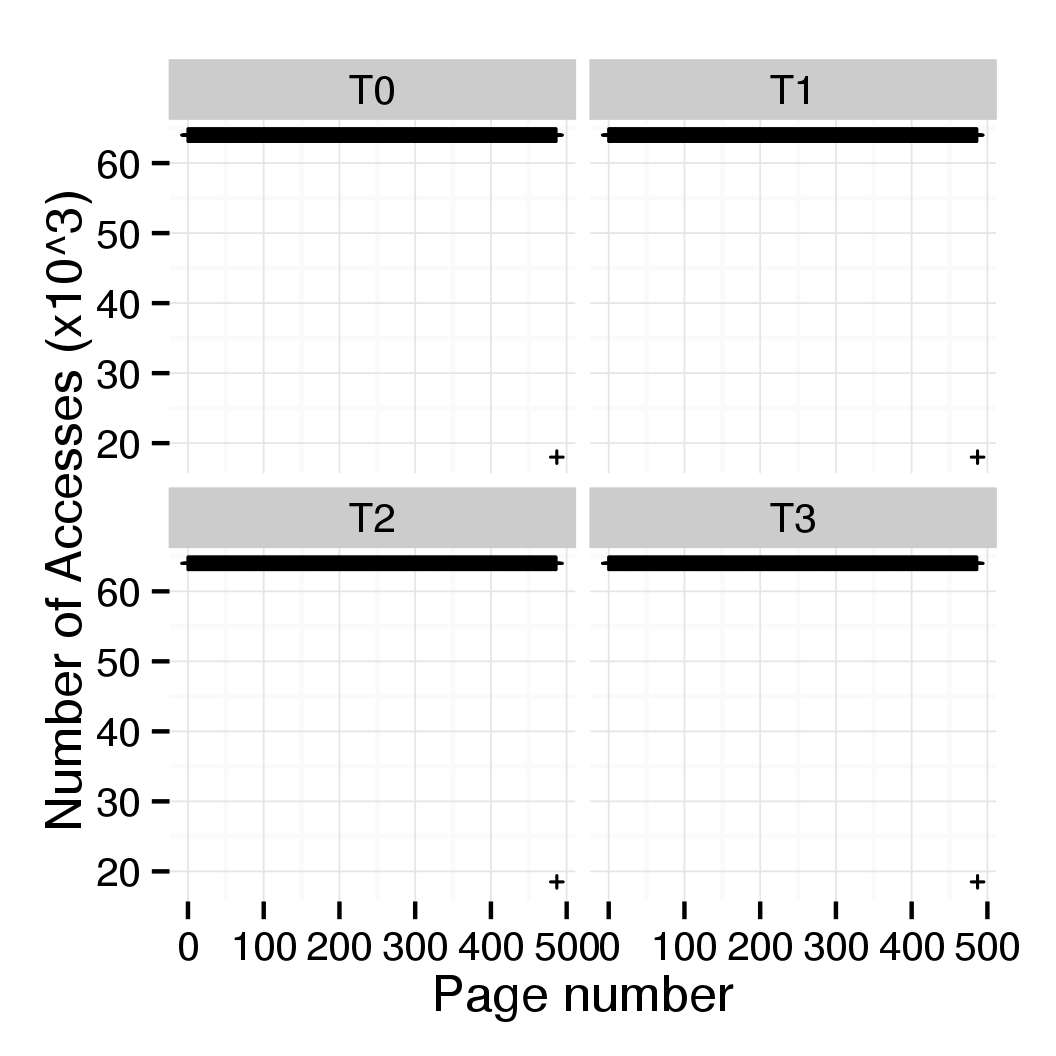
\includegraphics[height=.27\textheight] {mat_B_modulo}
        \label{fig:matrix-B-naive}
    }
    \subfigure[Structure C (naive)]{
        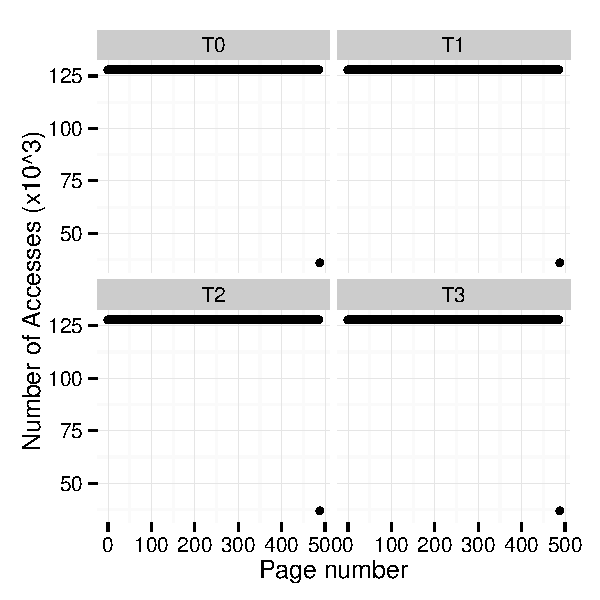
\includegraphics[height=.27\textheight] {mat_C_modulo}
        \label{fig:matrix-C-naive}
    }
    \caption{By thread access distribution on data structures A and B for the
        naive matrix multiplication. Each plots shows the number of access
    depending on the page number (inside the structure) for each thread.}
    \label{fig:matrix-naive}
\end{figure}

For the naive matrix multiplication, as we can see in
\ref{figure:matrix-naive}, all the pages of both structures are used by every
thread. Therefore, when we execute this code on a NUMA machine, wherever we
map the page, all the nodes but one will trigger remote memory accesses. We
can improve there are several ways to improve this behaviour: an easy solution
is to tell the operating system to interleave pages through the different
nodes. This will result on a better balance of memory bandwidth between the
nodes. An other solution is to create local copies of \texttt{A} and
\texttt{B} on each node as these matrix are only read. Finally we can modify
the algorithm to improve the locality, which mean using the bloc algorithm.

\DB{Experiment with local copy A,B?}

\begin{figure}[htb]
    \centering
    \subfigure[Structure B (bloc)]{
        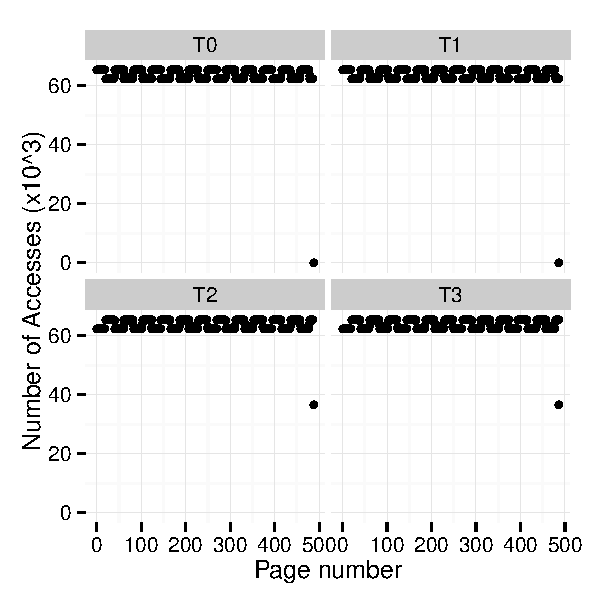
\includegraphics[height=.27\textheight] {mat_B_bloc}
        \label{fig:matrix-B-bloc}
    }
    \subfigure[Structure C (bloc)]{
        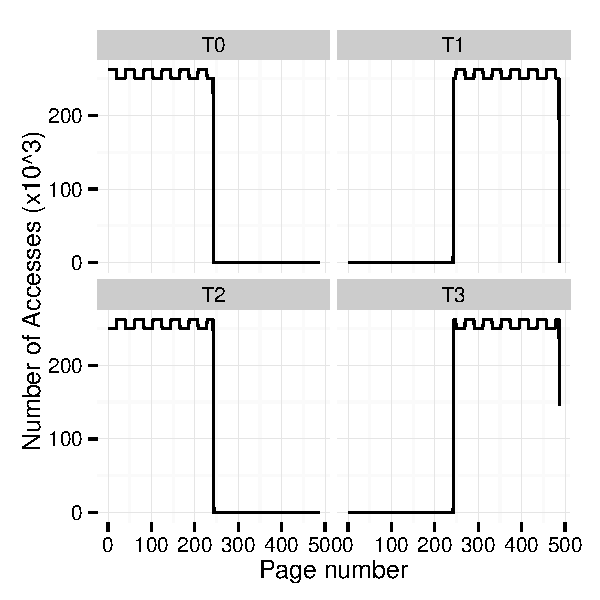
\includegraphics[height=.27\textheight] {mat_C_bloc}
        \label{fig:matrix-C-bloc}
    }
    \caption{By thread access distribution on data structures A and B for the
    bloc matrix multiplication.}
    \label{fig:matrix-bloc}
\end{figure}

As we can see in figure \ref{matrix-bloc}, the bloc algorithm improve the page
locality compared to the naive one. In our algorithm, structures
\texttt{B} and \texttt{C} are not divided the same way, resulting in two
different patterns. For structure \texttt{B} (fig \ref{fig:matrix-B-bloc}),
the pages are interleave, threads $T0$ and $T1$ works on the same pages while
threads $T2$ and $T3$ works on another set of pages. Structures \texttt{B} (and
\texttt{A}, fig \ref{fig:matrix-A-bloc}) are cut in two parts, the first half
is shared by thread $T0$ and $T2$ while the two others works on the second
half. This behaviour provides strong page exclusivity and is therefore more
suitable for NUMA machines. We can easily put each subpart of \texttt{C} (and
\texttt{A}) on a NUMA node and map the thread using it to this node, matrix
\texttt{B} can be distributed using interleave policy.


\DB{experiment description}
\begin{figure}[htb]
    \centering
    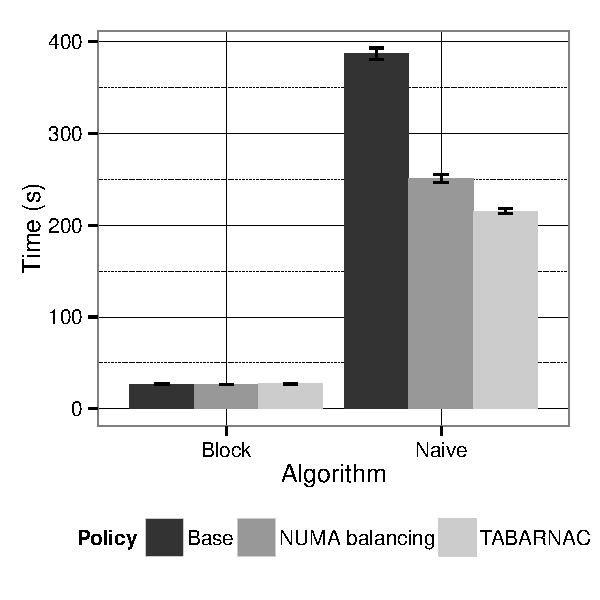
\includegraphics[width=.9\linewidth]{mat_time}
    \caption{Execution time of the matrix multiplication for size $4096*406$ doubles.}
    \label{fig:matrix-res}
\end{figure}

Results:
\begin{itemize}
    \item Big improvements for naive: better than every other tools
    \item Not that much for Bloc: algo designed to fit in cache figure
        \ref{fig:matrix-res}
    \item Cncl: \TABARNAC~ will help you modify code to do something like naive
        -> bloc if possible or at least to improve your NUMA mapping as for
        naive.
\end{itemize}

